\documentclass[12pt,letterpaper]{article}
\usepackage{fullpage}
\usepackage[top=2cm, bottom=4.5cm, left=2.5cm, right=2.5cm]{geometry}
\usepackage{amsmath,amsthm,amsfonts,amssymb,amscd}
\usepackage{lastpage}
\usepackage{enumerate}
\usepackage{fancyhdr}
\usepackage{mathrsfs}
\usepackage{xcolor}
\usepackage{graphicx}
\usepackage{listings}
\usepackage{hyperref}
\usepackage{tikz}
\usepackage{xfrac}
\usepackage{nicefrac}
\usepackage{xcolor}

\usetikzlibrary{shapes.geometric,fit}
\usetikzlibrary{patterns}

\hypersetup{
    colorlinks=true,
    linkcolor=blue,
    linkbordercolor={0 0 1}
}

\setlength{\parindent}{0.0in}
\setlength{\parskip}{0.05in}

\newcommand\course{ECON 3211}
\newcommand\hwnumber{7}
\newcommand\NetIDa{dc3451}
\newcommand\NetIDb{David Chen}

\theoremstyle{definition}
\newtheorem*{statement}{Statement}
\newtheorem*{claim}{Claim}
\newtheorem*{theorem}{Theorem}

\newcommand{\contra}{\Rightarrow\!\Leftarrow}
\newcommand{\Lag}{\mathcal{L}}

\pagestyle{fancyplain}
\headheight 35pt
\lhead{\NetIDa}
\lhead{\NetIDa\\\NetIDb}
\chead{\textbf{\Large Problem Set \hwnumber}}
\rhead{\course \\ \today}
\lfoot{}
\cfoot{}
\rfoot{\small\thepage}
\headsep 1.5em

\begin{document}

\section*{Problem 1}

\subsection*{a)}

The fixed costs don't vary with $q \implies FC = 200$.

The variable cost does vary with $q \implies VC = 0.1q^2 + 2q$.

$MC = \frac{dTC}{dq} = 0.2q + 2$.

$AVC = \frac{VC}{q} = 0.1q + 2$.

\subsection*{b)}
\begin{center}
  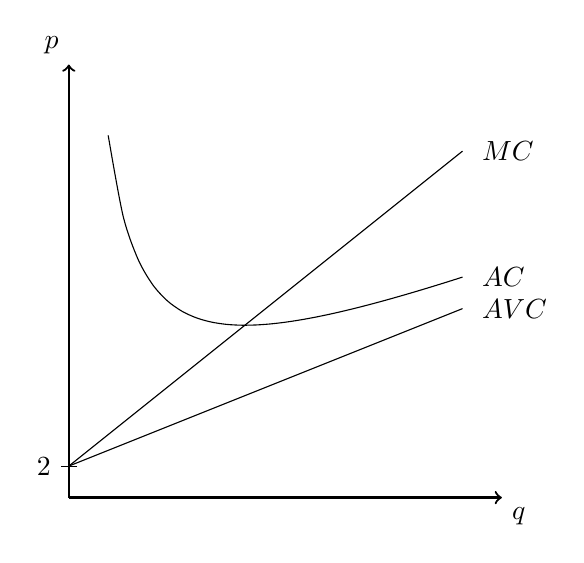
\begin{tikzpicture}[
    dot/.style={shape=circle, inner sep=2pt, draw, node contents=},
    circ/.style={shape=circle, inner sep=2pt, draw, fill}]
    \draw[thick,->] (0,0) -- (5.5,0) node[anchor=north west] {$q$};
    \draw[thick,->] (0,0) -- (0,5.5) node[anchor=south east] {$p$};

    \draw (3pt,0.4cm) -- (-3pt,0.4cm) node[anchor=east] {$2$}; 

    \draw[domain=0:100,scale=0.05,smooth,variable=\x] plot ({\x},{4*(0.2*\x + 2)}) node[label=right:{$MC$}]{};
    \draw[domain=0:100,scale=0.05,smooth,variable=\x] plot ({\x},{4*(0.1*\x + 2)}) node[label=right:{$AVC$}]{};
    \draw[domain=10:100,scale=0.05,smooth,variable=\x] plot ({\x},{4*(0.1*\x + 2 + 200/\x)}) node[label=right:{$AC$}]{};
  \end{tikzpicture}
\end{center}

\subsection*{c)}

The ``shut down'' price is the maximum price such that when a price taking firm
faces it, the profit-maximizing firm will close down. Assuming that in the short
run all fixed costs are sunk, we have that the shutdown price is $2$, which is
where the $MC$ curve is minimal at the corner.

However, if only $80\%$ is sunk, then we have that $AVC = 0.1q + 2 +
\frac{40}{q}$, and we see a shutdown at $\min(AVC) = 6$, as $\frac{dAVC}{dq} =
0.1 - \frac{40}{q^2} = 0 \implies q = 20 \implies \min(AVC) = 6$.

\subsection*{d)}

\begin{alignat*}{2}
  && \Pi(q) &= pq - 0.1q^2 - 2q - 200 \\
  &\implies& \frac{d\Pi}{dq} &= p - 0.2q - 2 = 0\\
  &\implies& q^* &= 5p - 10
\end{alignat*}

Since the wording of the problem is ambiguous, we have that if all fixed costs
are sunk, then this only holds if $p > 2$. If only $80\%$ are sunk, then this
holds only if $p > 2$. Thus, in the first case,

\[
  q(p) = \begin{cases}
    0 & p < 2 \\
    5p - 10 & p \geq 2
  \end{cases}
\]

In the second,

\[
  q(p) = \begin{cases}
    0 & p < 6 \\
    5p - 10 & p \geq 6
  \end{cases}
\]
\subsection*{e)}

The market supply is then $Q_s = 50q = 250p - 500$, if the price is above the
shut down price for each firm ($p > 2$ or $p > 6$).

\subsection*{f)}

We have that $Q_d = Q_s = Q^* = 3000-100P^* = 250P^* - 500 \implies 350P^* =
3500 \implies P^* = 10$. The firms open, so we have that $Q^* = 3000 - 100(10)
= 2000$, about $2000/50 = 40$ per firm.

\subsection*{g)}

\begin{center}
  \begin{tikzpicture}[
    dot/.style={shape=circle, inner sep=2pt, draw, node contents=},
    circ/.style={shape=circle, inner sep=2pt, draw, fill}]
    \draw[thick,->] (0,0) -- (8,0) node[anchor=north west] {$Q$};
    \draw[thick,->] (0,0) -- (0,8) node[anchor=south east] {$p$};

    \draw (3pt,0.5cm) -- (-3pt,0.5cm) node[anchor=east] {$2$}; 
    \draw (3pt,2.5cm) -- (-3pt,2.5cm) node[anchor=east] {$10$}; 
    \draw (2.5cm,3pt) -- (2.5cm,-3pt) node[anchor=north] {$2000$}; 

    \draw[dashed] (2.5,0) -- (2.5,2.5) -- (0,2.5);
    \draw[domain=2:25,scale=0.25,smooth,variable=\x] plot ({1.25*\x - 2.5},{\x}) node[label=right:{$S_{market}$}]{};
    \draw[domain=30:2,scale=0.25,smooth,variable=\x] plot ({15 - 0.5*\x},{\x}) node[label=right:{$D_{market}$}]{};
  \end{tikzpicture}
\end{center}

\subsection*{h)}

``Consumer surplus'' is a measure of consumer welfare. It can be interpreted as
the total difference between how much consumers are willing to pay and how much they
are actually paying. Critically, it varies similarly to compensating and
equivalent variation, but is not the same, being less clearly defined in terms
of utility.

In this market, since it is fairly simple, probably without varied price and
income changes that would make the approximate nature of CS important as a flaw.

\subsection*{i)}

Supply would be depressed to $Q_s = 250(p - 1) - 500 = 250p - 750$. The new
market equilibrium is then $Q_D = Q_S = 250P^* - 750 = 3000 - 100P^* \implies
P^* = \frac{3750}{350} = \frac{75}{7} \approx 10.71$. The price increases about
$71$ cents.

\subsection*{j)}

The quantity supplied is then $250\frac{75}{7} - 750 = \frac{13500}{7}$. At a
rate of \$1 per unit, we have that the total revenue is simply
$\$\frac{13500}{7} = \$1928.57$.

\subsection*{k)}

(Wait, it's $\pi$ for profit and not $\Pi$? Why does no one curl their lowercase $\pi$'s???)

Before the tax, we have that $\pi = pq - 0.1q^2 - 2q - 200 = 10(40) - 0.1(40^2)
- 2(40) - 200 = 400 - 160 - 80 - 200 = -40$. After the tax, we have that the new
quantity is $\frac{13500}{7(50)} = \frac{270}{7}$ per firm, which is also the
amount paid in taxes. Then, $\pi = pq -
0.1q^2 - 2q - 200 = \frac{75}{5}\frac{250}{7} - 0.1(\frac{250}{7})^2 -
2\frac{270}{7} - 200 - \frac{270}{7} \approx -51.22$. Profit decreases by about
11.22 after the tax.

\subsection*{l)}

Were I a souvenir store owner, I would post the pre-tax price and tell teh
consumer that the city collects a $\$1$ tax because the tax is likely not to be
fully salient. In that case, we would see that the extra $\$1$ tax is not
treated as a $\$1$ tax, but something less, meaning that consumers would be
willing to pay a higher price and also buy more, as the change in behaviour is
not as drastic as simply including the tax in the posted price.

\section*{Problem 2}

\subsection*{a)}

\begin{alignat*}{2}
  &\pi(q) &= pq - 100 - q -0.05q^2 \\
  &\implies& \frac{d\pi}{dq} &= p - 1 -0.1q = 0\\
  &\implies& q &= 10p - 10
\end{alignat*}

The market supply, given that there are 100 such firms, is then $Q_S = 100(10p-10) =
1000p - 1000$. Assuming that all fixed costs are sunk, the shutdown price is simply
$\$5$, as we have that $AVC = 1 + 0.05q \implies  \min(AVC) = 1$.

\subsection*{b)}

\begin{align*}
  \frac{p}{1} &= p = \frac{MU_q}{MU_M} \\
              &= \frac{9 - q}{1} \\
              &= 9 - q
\end{align*}

Thus, for the individual demand, we see that $p = 9 - q \implies q = 9 - p$.
Since we have that the total budget is $200$, we can always buy the amount of
$q$, as total expenditure is $pq = p(9-p)$, but $p, 9-p \geq 0 \implies 0 \leq p
\leq 9$, so $p(9-p) < 200$. Since there are 1000 such buyers, market demand is
then $Q_D = 1000(9-p) = 9000 - 1000p$.

\subsection*{c)}

\begin{center}
  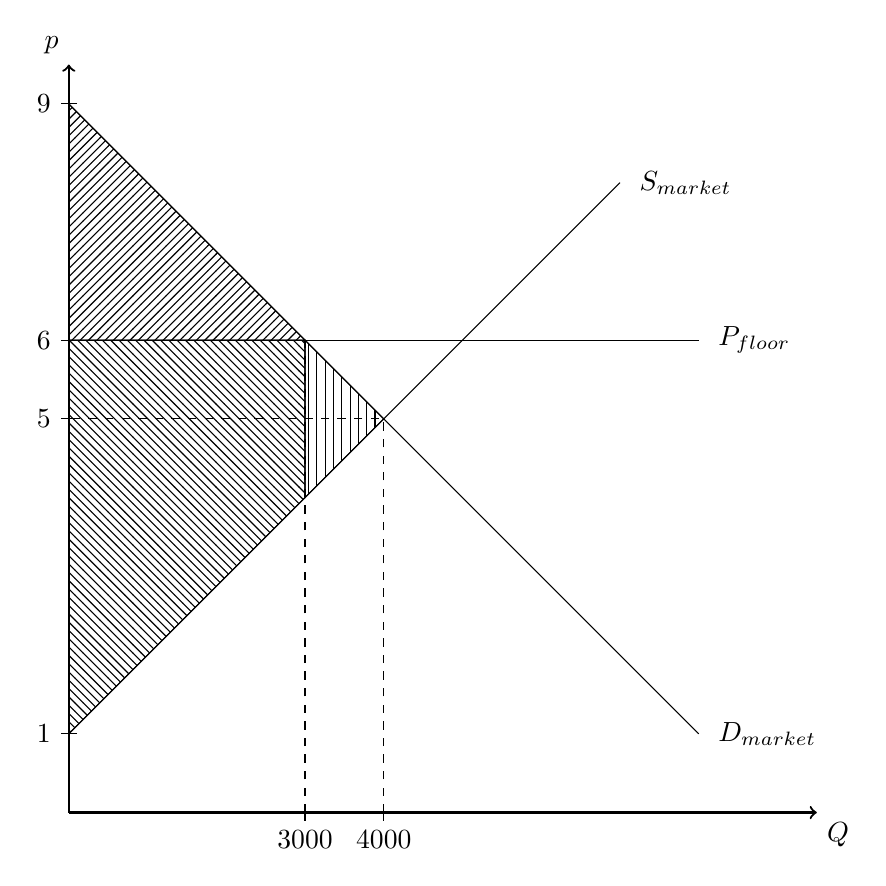
\begin{tikzpicture}[
    dot/.style={shape=circle, inner sep=2pt, draw, node contents=},
    circ/.style={shape=circle, inner sep=2pt, draw, fill}]
    \draw[thick,->] (0,0) -- (9.5,0) node[anchor=north west] {$Q$};
    \draw[thick,->] (0,0) -- (0,9.5) node[anchor=south east] {$p$};

    \draw (3pt,1cm) -- (-3pt,1cm) node[anchor=east] {$1$}; 
    \draw (3pt,9cm) -- (-3pt,9cm) node[anchor=east] {$9$}; 
    \draw (3pt,5cm) -- (-3pt,5cm) node[anchor=east] {$5$}; 
    \draw (3pt,6cm) -- (-3pt,6cm) node[anchor=east] {$6$}; 
    \draw (4cm,3pt) -- (4cm,-3pt) node[anchor=north] {$4000$}; 
    \draw (3cm,3pt) -- (3cm,-3pt) node[anchor=north] {$3000$}; 

    \draw[dashed] (4,0) -- (4,5) -- (0,5);
    \draw[dashed] (3,0) -- (3,6);
    \draw[domain=1:8,scale=1,smooth,variable=\x] plot ({\x - 1},{\x}) node[label=right:{$S_{market}$}]{};
    \draw[domain=9:1,scale=1,smooth,variable=\x] plot ({9-\x},{\x}) node[label=right:{$D_{market}$}]{};
    \draw (0,6) -- (8,6) node[label=right:{$P_{floor}$}]{};

    % \draw[fill=blue] (0,5) -- (0,6) -- (3,6) -- (3,5) -- cycle;
    % \draw[fill=red] (0,4) -- (0,5) -- (3,5) -- (3,4) -- cycle;
    % \draw[fill=green] (3,4) -- (3,6) -- (4,5);
    \draw[pattern=north west lines] (0,1) --(3,4) -- (3,6) -- (0,6) -- cycle;
    \draw[pattern=north east lines] (0,6) -- (3,6) -- (0,9) -- cycle;
    \draw[pattern=vertical lines] (3,4) -- (3,6) -- (4,5) -- cycle;
    % \draw[fill=gray!25!white]  (3,6) -- (4,6) -- (4,5) -- cycle;
  \end{tikzpicture}
\end{center}

\subsection*{d)}

We have that the equilibrium quantity is $Q^*= Q_D= Q_S = 9000 - 1000p = 1000p -
1000 \implies 2000p = 10000 \implies P^* = 5 \implies Q^* = 4000$.

\subsection*{e)}

The new equilibrium is $Q^* = 9000 - 1000(6) = 3000, P^* = 6$.

The consumer surplus is now decreased to the northeast line shaded area, which
has area less than the old surplus by $(1)(3000) +\frac{1}{2}(1000)(1) = 3500$. Similarly, the
producer surplus is increased to the northwest line shaded area, which has area
more than the old surplus by $1(3000) - \frac{1}{2}(1000)(1) = 5000 = 2500$.
Thus, while consumer surplus has decreased and producer surplus has increased,
overall surplus has decreased by 1000.

\subsection*{f)}

The price floor reduces market efficiency, as we have that total surplus has
decreased, meaning that the morket is not longer allocatively efficient, and we
can see that a deadweight loss of $\frac{1}{2}(1000)2 = 1000$ is incurred.

\section*{Problem 3}

\subsection*{a)}

$Q_S = Q_D = Q^* =2000 - 40P^* = 100P^* - 800 \implies 140P^* = 2800 \implies
P^* = 20, Q^* = 1200$.

\subsection*{b)}

Total expenditure in equilibrium is $P^*Q^* = 1200(20) =24000$.

\subsection*{c)}

The consumer surplus is a triangle, the area left of the demand curve above the
price. This has area $\frac{1}{2}(50-20)(1200) = 18000$. The producer surplus is
then also a triangle, the area left of the supply curve below the price. This
has area $\frac{1}{2}(20 -8)(1200) = 7200$.

\subsection*{d)}

If the government restricts to a quota of $Q = 800$, then we will see that the
loss in overall surplus is $\frac{1}{2}(30-16)(1200-800) = 2800$. This is since
the price pinned down by supply is $2000 - 40P = 800 \implies P = 30$, the price
pinned down by demand is $100P - 800 = 800 \implies P =16$. (This is clearer in
the graph).

\subsection*{e)}

\begin{center}
  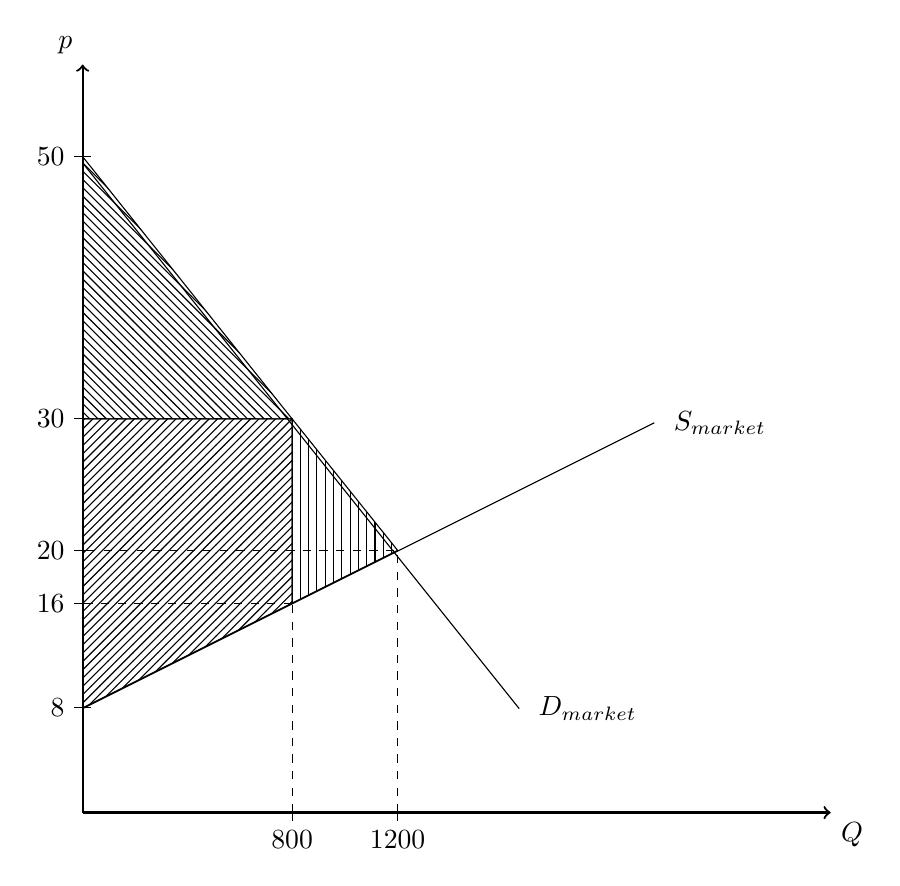
\begin{tikzpicture}[
    dot/.style={shape=circle, inner sep=2pt, draw, node contents=},
    circ/.style={shape=circle, inner sep=2pt, draw, fill}]
    \draw[thick,->] (0,0) -- (9.5,0) node[anchor=north west] {$Q$};
    \draw[thick,->] (0,0) -- (0,9.5) node[anchor=south east] {$p$};

    % \draw (3pt,1cm) -- (-3pt,1cm) node[anchor=east] {$1$}; 
    \draw (3pt,5cm) -- (-3pt,5cm) node[anchor=east] {$30$}; 
    \draw (3pt,3.33cm) -- (-3pt,3.33cm) node[anchor=east] {$20$}; 
    \draw (3pt,2.66cm) -- (-3pt,2.66cm) node[anchor=east] {$16$}; 
    \draw (3pt,1.33cm) -- (-3pt,1.33cm) node[anchor=east] {$8$}; 
    \draw (3pt,8.33cm) -- (-3pt,8.33cm) node[anchor=east] {$50$}; 
    \draw (4cm,3pt) -- (4cm,-3pt) node[anchor=north] {$1200$}; 
    \draw (2.66cm,3pt) -- (2.66cm,-3pt) node[anchor=north] {$800$}; 

    \draw[dashed] (4,0) -- (4,3.33) -- (0,3.33);
    \draw[dashed] (2.66,0) -- (2.66,5) -- (0,5);
    \draw[dashed] (2.66,2.66) -- (0,2.66);
    % \draw[dashed] (4,0) -- (4,5) -- (0,5);
    % \draw[dashed] (3,0) -- (3,6);
    \draw[domain=8:30,scale=0.33,smooth,variable=\x] plot ({\x - 8},{0.5*\x}) node[label=right:{$S_{market}$}]{};
    \draw[domain=50:8,scale=0.33,smooth,variable=\x] plot ({20-0.4*\x},{0.5*\x}) node[label=right:{$D_{market}$}]{};
    % \draw () -- (8,6) node[label=right:{$P_{floor}$}]{};

    \draw[pattern=north west lines] (0,5) -- (2.66,5) -- (0,8.33) -- cycle;
    \draw[pattern=north east lines] (0,1.33) -- (2.66,2.66) -- (2.66,5) -- (0,5) -- cycle;
    \draw[pattern=vertical lines] (2.66,2.66) -- (2.66,5) -- (4,3.33) -- cycle;
  \end{tikzpicture}
\end{center}

The northwest shaded lines are consumer surplus if the price settles at $P
=30$, and the northeast lines producer surplus. The vertical lines show
deadweight loss, or the loss in total surplus.

\subsection*{f)}

The loss in total surplus is not affected by where the final price lands, so
long as it lands in the range $[16,30]$ and all the firms stay open. However,
consumer surplus is maximized at $P = 16$ and minimized $P = 30$, with increases
and decreases in producer surplus offsetting any decreases and increases in
consumer surplus due to a change in the price. Intuitively, this makes sense, as
the sum will be the same shape on the graph irregardless of the price, so long
as it is in that range that makes $Q = 800$.

\subsection*{g)}

Algebraically, we have that $CS = \frac{1}{2}(800)(50 - P  + 30 - P) = 400(80 -
2P), PS = \frac{1}{2}(800)(P - 16 + P - 8) = 400(2P  - 24)$. Then, $CS + PS =
400(80 - 24 + 2P - 2P) = 400(56) = 38400$. 

\section*{Problem 4}

\subsection*{a)}
\subsubsection*{a.1}

The minimum efficient scale at which the firm will operate is that $MC = AC
\implies 0.2q + 2 = 0.1q + 2 + \frac{160}{q} \implies 0.1q = \frac{160}{q}
\implies q_{MES} = 40$.

Thus, minimum efficient scale is producing $40$ units.

\subsubsection*{a.2}

The average total cost is $0.1(40) + 2 + \frac{160}{40} = 4 + 2 + 4 = 10$.

\subsubsection*{a.3}

In the long run, price will prevail at $10$, as we have that if $p < 10$, firms
will make economic losses and exit until normal profit is achieved at $p = 10$.
Similarly, we have that if $p > 10$, firms will enter until price is depressed
to $p = 10$.

\subsection*{b)}

We have that since each firm supplies 40 units, market equilibrium supply is
$40n$, where $n$ is the number of firms. $Q^D = Q^* = 40n = 3200 - 100P = 3200 -1000 = 2200 \implies
n = 55$.

\subsection*{c)}

The short run supply function of the firm is $\pi(q) = pq - 0.1q^2 - 2q - 160
\implies \frac{d\pi}{dq} = p - 0.2q - 2 = 0 \implies q = 5p - 10$.

\subsection*{d)}

The market supply in the short run, if there are 55 firms, is $Q_S = 55q = 275p - 550$.

\subsection*{e),f),g)}

\begin{center}
  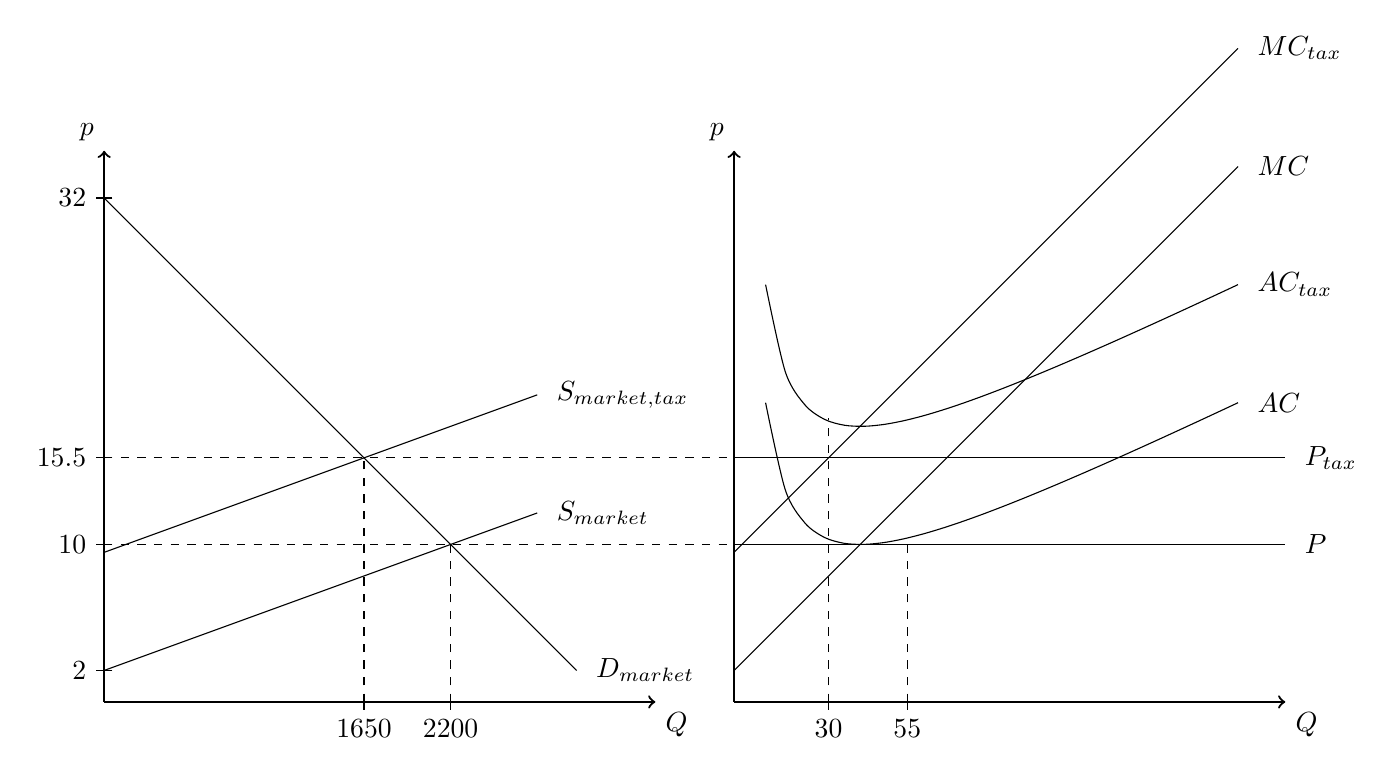
\begin{tikzpicture}[
    dot/.style={shape=circle, inner sep=2pt, draw, node contents=},
    circ/.style={shape=circle, inner sep=2pt, draw, fill}]
    \draw[thick,->] (0,0) -- (7,0) node[anchor=north west] {$Q$};
    \draw[thick,->] (0,0) -- (0,7) node[anchor=south east] {$p$};

    % \draw (3pt,1cm) -- (-3pt,1cm) node[anchor=east] {$1$}; 
    \draw (3pt,6.4cm) -- (-3pt,6.4cm) node[anchor=east] {$32$}; 
    \draw (3pt,0.4cm) -- (-3pt,0.4cm) node[anchor=east] {$2$}; 
    \draw (3pt,2cm) -- (-3pt,2cm) node[anchor=east] {$10$}; 
    \draw (3pt,3.1cm) -- (-3pt,3.1cm) node[anchor=east] {$15.5$}; 
    % \draw (3pt,1.33cm) -- (-3pt,1.33cm) node[anchor=east] {$8$}; 
    % \draw (4cm,3pt) -- (4cm,-3pt) node[anchor=north] {$1200$}; 
    \draw (4.4cm,3pt) -- (4.4cm,-3pt) node[anchor=north] {$2200$}; 
    \draw (3.3cm,3pt) -- (3.3cm,-3pt) node[anchor=north] {$1650$}; 
    \draw (10.2cm,3pt) -- (10.2cm,-3pt) node[anchor=north] {$55$}; 
    \draw (9.2cm,3pt) -- (9.2cm,-3pt) node[anchor=north] {$30$}; 

    % \draw[dashed] (4,0) -- (4,3.33) -- (0,3.33);
    % \draw[dashed] (2.66,0) -- (2.66,5) -- (0,5);
    % \draw[dashed] (2.66,2.66) -- (0,2.66);
    % \draw[dashed] (4,0) -- (4,5) -- (0,5);
    % \draw[dashed] (3,0) -- (3,6);
    \draw[dashed] (0,2) -- (8,2);
    \draw[dashed] (4.4,0) -- (4.4,2);
    \draw[dashed] (0,3.1) -- (8,3.1);
    \draw[dashed] (3.3,0) -- (3.3,3.1);
    \draw[dashed] (10.2,0) -- (10.2,2);
    \draw[dashed] (9.2,0) -- (9.2,3.6);
    \draw (8,3.1) -- (15,3.1) node[label=right:{$P_{tax}$}]{};
    \draw (8,2) -- (15,2) node[label=right:{$P$}]{};
    \draw[domain=2:12,scale=0.2,smooth,variable=\x] plot ({2.75*\x - 5.5},{\x}) node[label=right:{$S_{market}$}]{};
    \draw[domain=2:12,scale=0.2,smooth,variable=\x] plot ({2.75*\x - 5.5},{\x + 7.5}) node[label=right:{$S_{market,tax}$}]{};
    \draw[domain=32:2,scale=0.2,smooth,variable=\x] plot ({32-\x},{\x}) node[label=right:{$D_{market}$}]{};
    % \draw () -- (8,6) node[label=right:{$P_{floor}$}]{};

    % \draw[pattern=north west lines] (0,5) -- (2.66,5) -- (0,8.33) -- cycle;
    % \draw[pattern=north east lines] (0,1.33) -- (2.66,2.66) -- (2.66,5) -- (0,5) -- cycle;
    % \draw[pattern=vertical lines] (2.66,2.66) -- (2.66,5) -- (4,3.33) -- cycle;

    \draw[thick,->] (8,0) -- (15,0) node[anchor=north west] {$Q$};
    \draw[thick,->] (8,0) -- (8,7) node[anchor=south east] {$p$};

    \draw[domain=10:160,scale=0.2,smooth,variable=\x] plot ({\x / 5 + 40},{0.1*\x + 2 + 160/\x}) node[label=right:{$AC$}]{};
    \draw[domain=0:160,scale=0.2,smooth,variable=\x] plot ({\x / 5 + 40},{0.2*\x + 2}) node[label=right:{$MC$}]{};
    \draw[domain=0:160,scale=0.2,smooth,variable=\x] plot ({\x / 5 + 40},{0.2*\x + 2 + 7.5}) node[label=right:{$MC_{tax}$}]{};
    \draw[domain=10:160,scale=0.2,smooth,variable=\x] plot ({\x / 5 + 40},{0.1*\x + 2 + 7.5 + 160/\x}) node[label=right:{$AC_{tax}$}]{};
    
  \end{tikzpicture}
\end{center}

The post tax equilibrium is seen by solving $275(P - 7.5) - 550 = 3200 - 100P$.

\subsection*{h)}

The firms no longer make a profit in the short run, but still produce since they
are above shutdown price if all fixed costs are sunk - this is given by $AVC =
0.1q + 2 < MC = 0.2q + 2$.

In the long run, firms will exit until supply is depressed to the point that
price is at the minimum efficient scale for the firms, and economic profit is 0.

\subsection*{i)}

Since the long run supply curve is infinitely elastic, in the long run we will
see that the entire incidence of the tax falls onto consumers, with this trend
being more and more true as more and more firms exit the market, as this brings
price closer to the minimum efficient level. This reduces consumer surplus, but
producer surplus is fixed at 0 in the long run.

\section*{Problem 5}

(Does this include the tax? Unclear)

\subsection*{a)}

The minimum efficient scale now occurs at $MC = AC \implies 0.2q + 2 = 0.1q + 2
+ \frac{360}{q} \implies 0.1q = \frac{360}{q} \implies q_{MEC} = 60$. The firm must
produce more to be efficient.

\subsection*{b)}

The long term price will then also rise, as firms will exit until price faced by
the firms is equal to $AC_{MEC} = 0.1(60) + 2 + \frac{360}{60} = 6 + 2 + 6 = 14.$

\subsection*{c)}

The introduction of the licensing fee reduces the amount of firms in the
industry. This is because we have prices rise, indicating that the market
quantity demanded will diminish, but firms at minimal efficient scale - as they
are in the long run - must produce more. Thus, firms must exit to keep market
supply consistent with market demand.

Specifically, we see that $q_d = 3200 - 100(14) = 60n \implies n = 30$ firms in
the market in the long run.

\subsection*{d)}

The government collects $200$ each from $30$ firms, so $6000$ total in revenue.

\subsection*{e)}

The licensing fee must reduce consumer surplus, as the price is raised, and
consumer surplus is the area left of demand above price. 

\subsection*{f)}

In the long run, the entire incidence falls onto consumer and thus the market
price will settle at $14$.

\subsection*{g)}

The long run equilibrium quantity will fall to $Q_D = 3200 - 14(100) = 1800$,
same as the lump sum tax case, raising $1800(4) = 7200$ in revenue.

\subsection*{h)}

The policies arrive at the same equilibrium, but raise different amounts of
revenue. They therefore aren't equivalent policies, but also they also have
noncongruent effects on whether firms shut down in the short run, for example.
The lump sum tax doesn't change variable costs, but the per-unit one does,
meaning that firms are more likely to shut down in the short term when facing a
lump sum tax.

\end{document}